\section{Software}
\textbf{Hinweise zur Benutzung}\\
Der Fachbericht dient zur Erklärung des Aufbaus des Java Source Codes. Für eine Einführung in das Programm beachte man die Bedienungsanleitung im Anhang.\\
\textit{JavaKlassenNamen} sind im Folgenden kursiv mit Grossbuchstaben geschrieben. Dagegen sind \textit{packages} kursiv und klein geschrieben. Das gesamte Klassendiagramm befindet sich im Anhang.\\
Fett gedruckte Nummern (\textbf{1}) beziehen sich auf Elemente des GUIs. Eine Abbildung des GUIs mit Nummerierung findet sich am Ende der Bedienungsanleitung im Anhang.\\

\textbf{Ziele}\\
Ziel der Applikation ist die automatische Dimensionierung eines Reglers mit der Phasengangmethode von Prof. J. Zellweger. Weiter soll die Schrittantwort des gesamten Regelkreises ermittelt und visualisiert werden. Die Regelstrecke ist durch die Parameter $K_s$, $T_u$ und $T_g$ gegeben. Neben der Phasengangmethode sind auch Faustregeln zur Reglerdimensionierung anwendbar. Die berechneten Werte sowie die markanten Werte der Schrittantwort sollen als Text ausgegeben werden. Die Software verfügt weiter über die nützlichen Befehle Rückgängig und Wiederholen. Die eingegebenen Werte können zudem gespeichert und geladen werden.\\

\textbf{Aufbau und Packages}\\
Die Applikation ist nach dem Model-View-Controller Architekturmuster aufgebaut. Wiedergespiegelt ist das in den drei Packages \textit{model}, \textit{view} und \textit{controller}.\\
Das \textit{model} soll eine Abstraktion der mathematischen Objekte bieten. Die meisten enthaltenen Klassen sind für die Vermeidung von Aliasing-Problemen (Zugriff zweier Klassen auf die gleiche Instanz) als unveränderlich gehalten.\\
Die Klassen zur Reglerdimensionierung sind für die bessere Kapselung im separaten Package \textit{model.dimensionierung} enthalten. Alle Klassen dieses Packages sind als unveränderlich gehalten.\\
Das \textit{view} erzeugt die graphische Benutzeroberfläche mit den Daten des \textit{models}. Die Kommunikation zwischen \textit{view} und \textit{model} erfolgt mittels dem Observer Entwurfsmuster.\\
Der \textit{controller} übernimmt die Steuerung der Applikation und die Ausführung der Befehle des Benutzers. 


\newpage
\subsection{Packages und ihre Klassen}

\subsubsection{Klassen des Packages \textit{controller}}
Der Aufbau des Packages \textit{controller} ist in Abbildung \ref{packcontrl} ersichtlich.\\

\textit{\textbf{Controller}}\\
Der \textit{Controller} ist verantwortlich für die Steuerung der Applikation. Er besitzt für alle Befehle die der Benutzer im GUI tätigen kann eine Methode zur Modifizierung des \textit{Models}. Meldet das \textit{Model} beim Modifizieren einen Fehler informiert er den Benutzer mit der Methode displayError des \textit{Views}. Vor jeder Änderung des \textit{Models} speichert sich der \textit{Controller} eine Kopie davon. Dadurch ist es möglich alte Zustände wiederherzustellen und die Befehle Rückgängig und Wiederholen zu unterstützen. Weiter ist der \textit{Controller} für das Speichern und Laden zuständig. Dies funktioniert da das \textit{Model} das \textit{Serializable} Interface implementiert und der \textit{Controller} so die Daten mit einem \textit{ObjectOutputStream} in eine Datei schreiben bzw. mit einem \textit{ObjectInputStream} aus einer Datei laden kann.\\

\textit{\textbf{PIDRechner}}\\
Diese Klasse ist der Startpunkt (main) der Applikation. Sie initialisiert \textit{Controller}, \textit{View} und \textit{Model}.

\begin{figure}[p]
\centering
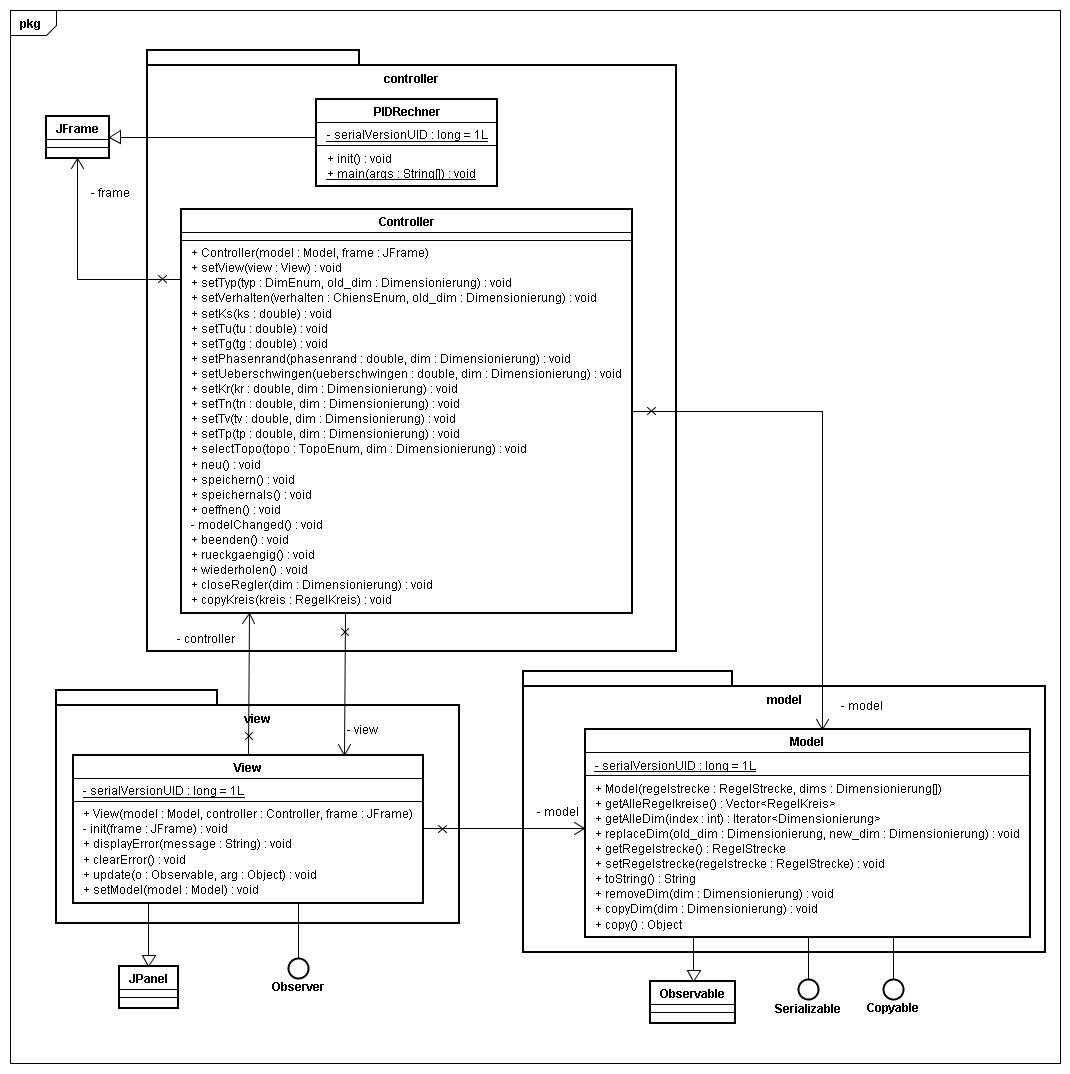
\includegraphics[width=1\textwidth]{packcontrl.png}
\caption{Package \textit{controller}}
\label{packcontrl}
\end{figure}

\newpage
\subsubsection{Ausgewählte Klassen des Packages \textit{model}}
Der Aufbau des Packages \textit{model} ist in Abbildung \ref{packmodel} ersichtlich.\\

\textit{\textbf{Model}}\\
Das \textit{Model} verwaltet die \textit{Regelstecke} und die verschiedenen \textit{Dimensionierungen}. Es bietet Zugriffsmethoden um die \textit{Regelstrecke} und \textit{Dimensionierungen} zu modifizieren. Auch kann es Dimensionierungsmethoden kopieren oder löschen.\\

\textit{\textbf{Regelkreis}}\\
Die Klasse \textit{Regelkreis} dient zur Umwandlung der Übertragungsfunktionen (\textit{TransferFunction}) von Regelstrecke und Regler in die Übertragungsfunktion des ganzen Kreises.\\

\textit{\textbf{Regelstrecke}}\\
Die Klasse \textit{Regelstrecke} bietet eine Abstraktion einer PTn-Strecke mit den Attributen $K_s$, $T_u$ und $T_g$. Eine \textit{Regelstrecke} ist ein \textit{Regelglied}, das heisst sie kann als eine Übertragungsfunktion angesehen werden. Die Übertragungsfunktion wird durch die Sani-Approximation (\textit{SaniApprox}) gebildet.\\

\textit{\textbf{Regler}}\\
Diese Klasse dient zur Abstraktion eines PID-T Reglers mit den Parametern $K_R$, $T_n$, $T_v$ und $T_p$. Ein \textit{Regler} wird normalerweise durch eine Dimensionierungsmethode (\textit{Dimensionierung}) gebildet.\\

\textit{\textbf{TransferFunction}}\\
Eine Übertragungsfunktion besteht aus Zähler- und Nenner-\textit{Polynom}. Sie bietet Methoden zur Faltung und Berechnung der Residuen. Weiter kann aus jeder Übertragungsfunktion eine \textit{Schrittantwort} gebildet werden.\\

\textit{\textbf{Polynom}}\\
\textit{Polynom} abstrahiert reelle Polynome beliebigen Grades. Es bietet Methoden zur Addition und Multiplikation mit anderen \textit{Polynomen}. Weiter können die Wurzeln und die Residuen (mit einem angenommenen Zähler von 1) ausgelesen werden. \\
 
\textit{\textbf{Schrittantwort}}\\
Die Klasse \textit{Schrittantwort} stellt die Schrittantwort für ein lineares \textit{Regelglied} ohne Durchgriff dar. Sie bietet zudem Methoden zur Analyse. So kann sie feststellen ob eine Schrittantwort ausschwingt und wie gross An- und Ausschwingzeit sind. Weiter sucht sie nach dem Maximalwert der Kurve und bietet die Möglichkeit dessen Zeitpunkt und Grösse auszulesen.

\begin{figure}[p]
\centering
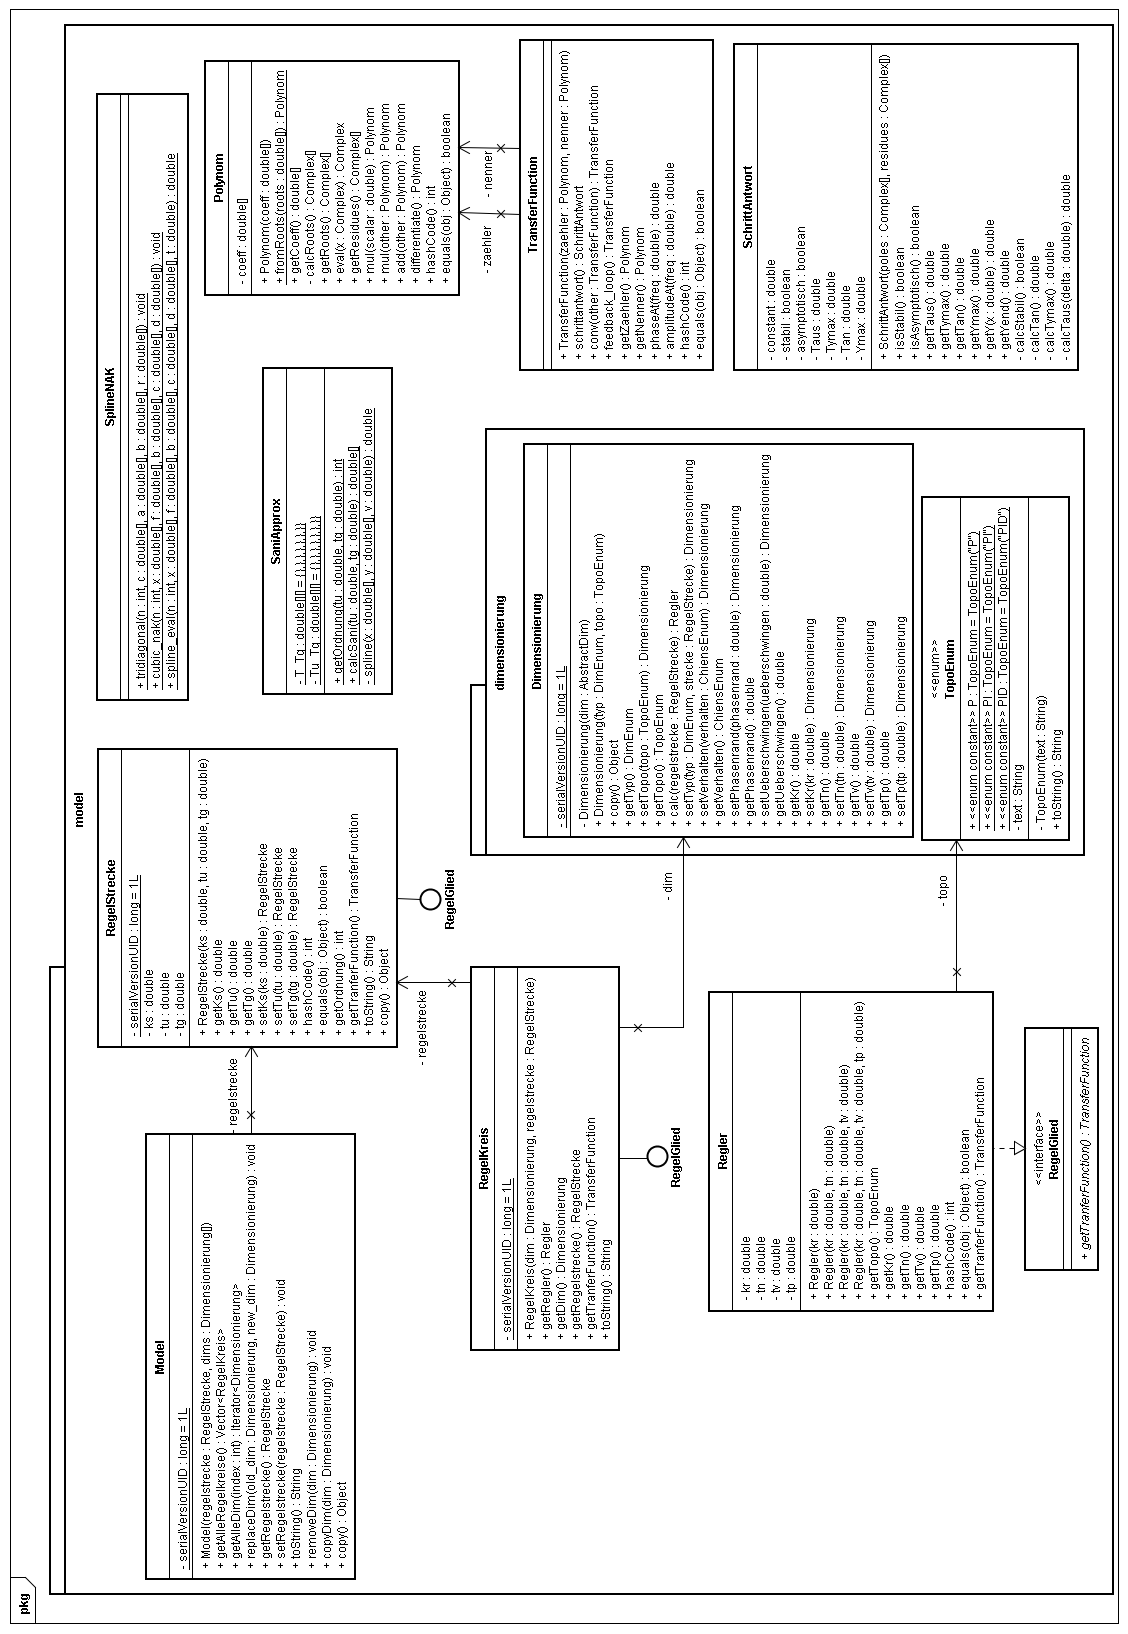
\includegraphics[width=1\textwidth]{packmodel.png}
\caption{Package \textit{model}}
\label{packmodel}
\end{figure}

\newpage
\subsubsection{Ausgewählte Klassen des Packages \textit{dimensionierung}}
Der Aufbau des Packages \textit{dimensionierung} ist in Abbildung \ref{packdim} ersichtlich.\\

\textit{\textbf{Dimensionierung}}\\
Diese Klasse ist eine Auswahl der anderen Dimensionierungsarten, wobei immer nur eine Dimensionierungsart aktiv ist. So bietet diese Klasse auch alle Methoden der anderen Dimensionierungsmethoden. Wird eine Methode bei einer falschen Variante verwendet, wirft die Klasse eine \textit{ClassCastException}. Der Typ (\textit{DimEnum}) kann mit der Methode setTyp gewechselt werden. Beim Wechseln zu der Manuellen Dimensionierungsmethode, werden die Werte des dimensionierten Reglers übernommen.\\

\textit{\textbf{DimEnum}}\\
Dieser Enum dient zur Aufzählung aller Dimensionierungstypen. Er ordnet jedem Typ auch einen Text zu.\\

\textit{\textbf{TopoEnum}}\\
Zur Unterscheidung von PI- und PID-Reglern wird dieser Enum verwendet.\\

\textit{\textbf{AbstractDim}}\\
\textit{AbstractDim} ist die abstrakte Grundklasse aller Dimensionierungsmethoden. Die Methode calc berechnet für eine gegebene Regelstrecke einen Regler. Durch get- und setTopo lässt sich die Reglertopologie (\textit{TopoEnum}) modifizieren. Die Methode getTyp() gibt den Typ des konkreten \textit{Reglers} zurück.\\

\textit{\textbf{ZellwegerDim}}\\
Hier steckt die Phasengangmethode zur Reglerdimensionierung. Die Beschreibung der Methode findet sich im theoretischen Teil.\\

\textit{\textbf{IterativDim}}\\
Diese Methode führt die Phasengangmethode (\textit{ZellwegerDim}) mehrmals nacheinander aus und sucht mit einer binären Suchmethode nach dem gewünschten Überschwingen der Schrittantwort.\\

Die restlichen Klassen entsprechen den verschiedenen Faustregeln.

\begin{figure}[p]
\centering
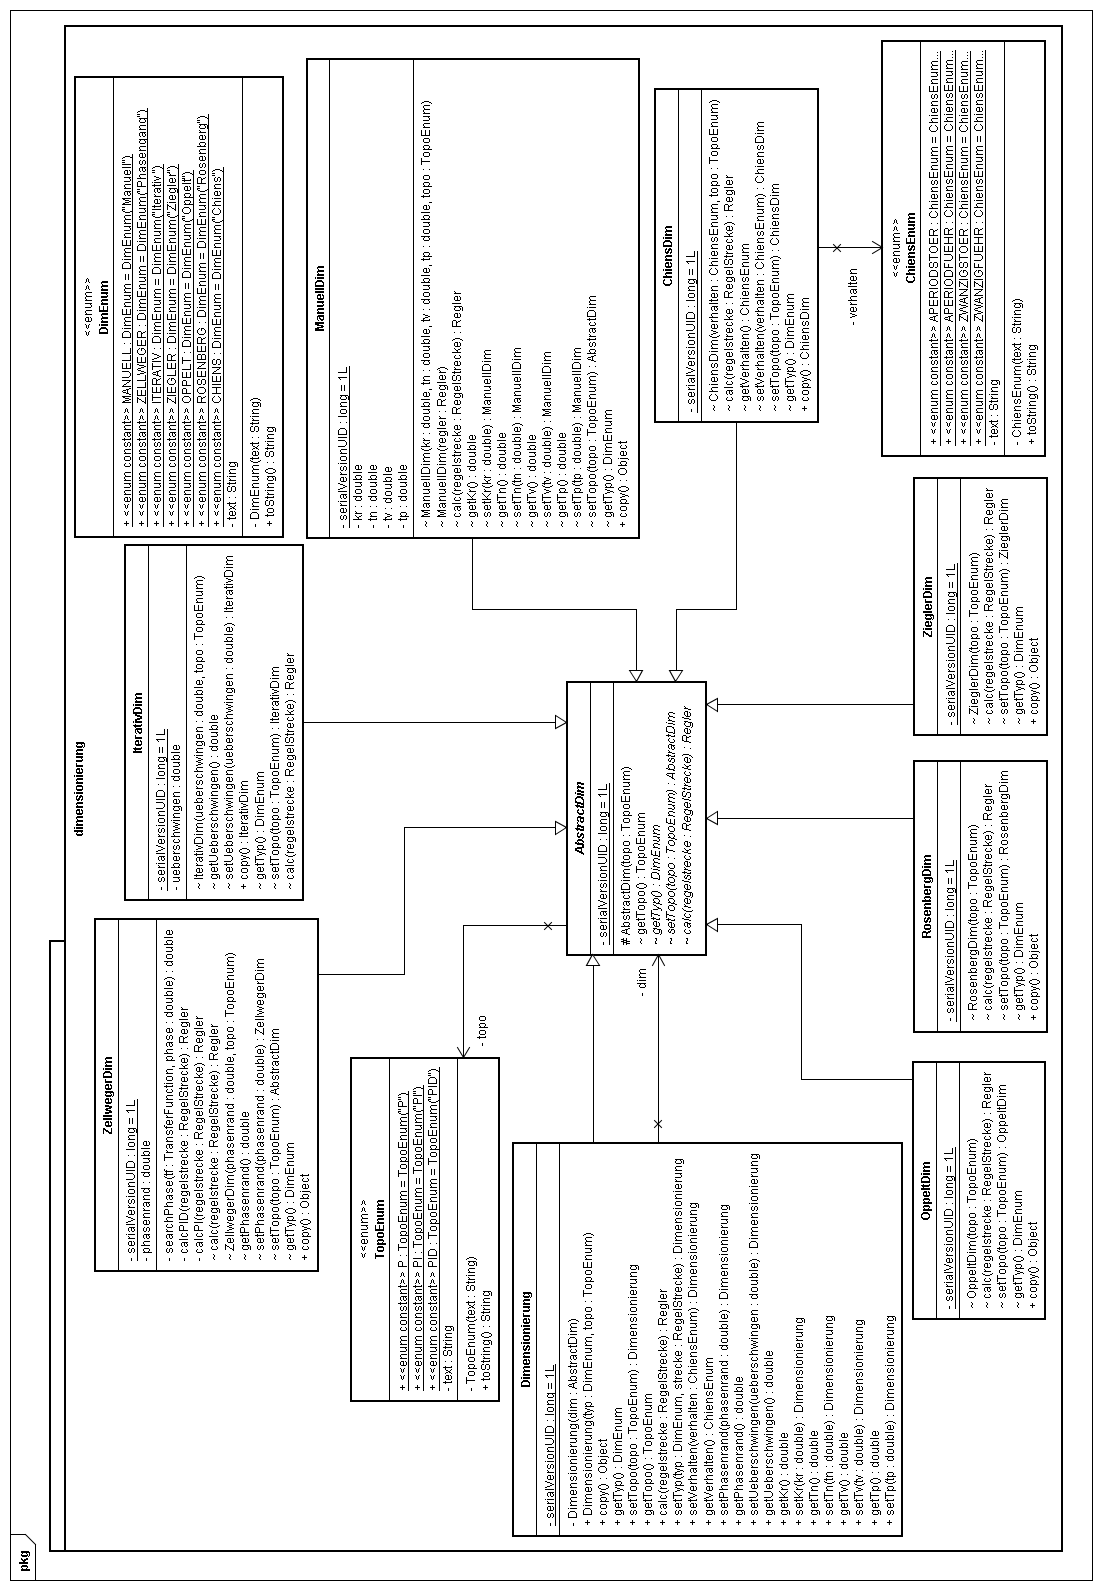
\includegraphics[width=1\textwidth]{packdim.png}
\caption{Package \textit{dimensionierung}}
\label{packdim}
\end{figure}

\newpage
\subsubsection{Klassen des Packages \textit{view}}
Der Aufbau des Packages \textit{view} ist in Abbildung \ref{packview} ersichtlich.\\

\textit{\textbf{View}}\\
\textit{View} ist die oberste Ebene im GUI (abgesehen vom \textit{JFrame}). Es beheimatet die \textit{Sidebar}, den \textit{Graph} und die Statuszeile. Auch initialisiert es die Menübar vom \textit{JFrame}.\\

\textit{\textbf{SidebarPanel}}\\
\textit{SidebarPanel} ordnet die einzelnen Panels von \textit{RegelstreckeView}, \textit{ReglerView} und \textit{AnalyseView} vertikal untereinander an. Es können mehrere Instanzen von \textit{ReglerView} angezeigt werden.\\

\textit{\textbf{RegelstreckeView}} (\textbf{1})\\
\textit{RegelstreckeView}  zeigt die Parameter der \textit{Regelstrecke} sowie die berechnete Ordnung und die Zeitkonstanten an.\\

\textit{\textbf{ReglerView}} (\textbf{2})\\
Dieses \textit{JPanel} visualisiert den Typ der Dimensionierungsmethode, deren Parameter und die Werte des daraus resultierenden \textit{Reglers}.\\

\textit{\textbf{AnalyseView}} (\textbf{3})\\
Listet die Eigenschaften Anstiegszeit ($T_{an}$), Ausschwingzeit ($T_{aus}$), Maximalwert ($Y_{max}$) und Zeitpunkt des Maximalwertes ($T_{Ymax}$) der \textit{Schrittantwort} auf.\\

\textit{\textbf{Graph}} (\textbf{4})\\
Zeichnet alle \textit{Schrittantworten} mit der Klasse \textit{ChartPanel} von JFreeChart. Unter dem Graphen zeigt es weiter eine Legende. Die Zustände der \textit{Checkboxen} werden nur vom Graph selbst verwendet und nicht dem \textit{Controller} mitgeteilt.

\begin{figure}[p]
\centering
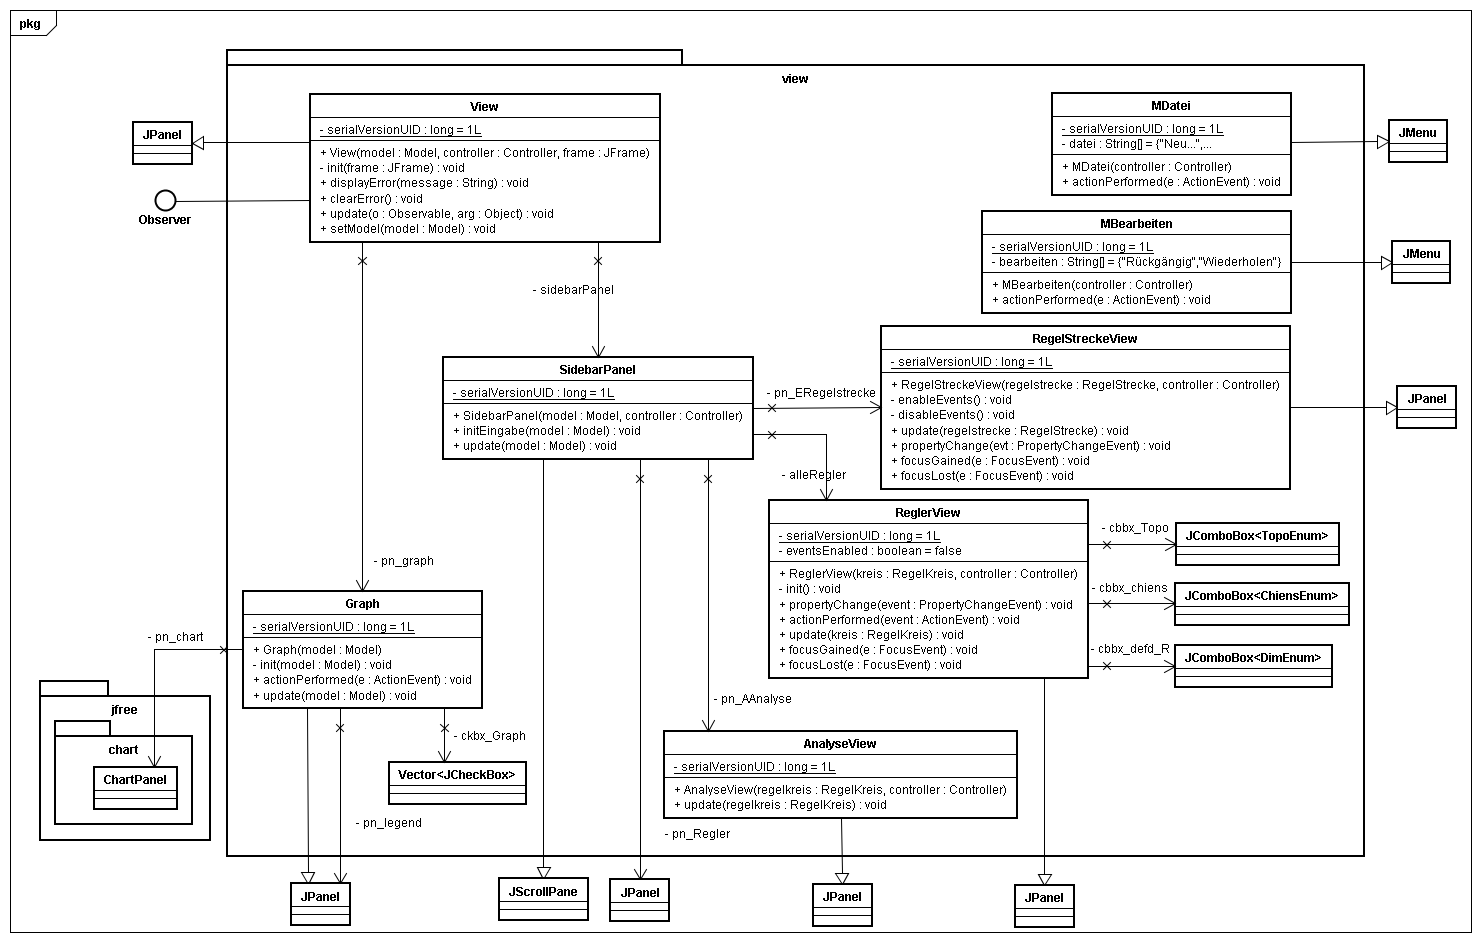
\includegraphics[width=0.9\textwidth]{packview.png}
\caption{Package \textit{view}}
\label{packview}
\end{figure}

\newpage
\subsection{Benutzerinteraktion}
Vorgaben: Das Programm wurde gestartet und im Eingabefeld $T_u$ wurde der Wert 1.0 eingegeben. Weiter wurde als Dimensionierungsart Iterativ ausgewählt. Nun gibt man im Eingabefeld $T_g$ den Wert 1.6 ein. Dadurch wird folgender Ablauf gestartet:\\
\begin{itemize}
\item In der Klasse \textit{RegelStreckeView} wird durch das System die Methode propertyChange des \textit{PropertyChangeListeners} aufgerufen. Es wird die Quelle des Events überprüft und festgestellt, dass es von dem Textfeld für $T_g$ kommt. Danach wird der Zahlenwert des Textfeldes eingelesen und an die Methode setTg vom \textit{Controller} weitergeleitet.\\
\item Der \textit{Controller} macht sich eine Kopie des \textit{Models} und speichert sich diese auf einem Stack. Danach bildet er sich eine neue \textit{Regelstrecke} mit der Methode setTg von der alten \textit{Regelstrecke}. Nun setzt der \textit{Controller} mit der Methode setRegelstrecke die Regelstrecke des \textit{Models} auf die neue Instanz, dabei wird als Nebeneffekt die Methode update vom \textit{View}, welches ein Observer ist, aufgerufen. \\ 
\item Das \textit{View} ruft nun die Methode update von den beiden Klassen \textit{SideBarPanel} und \textit{Graph} auf.\\
\item Die update Methode vom \textit{SideBarPanel} ruft update von \textit{RegelStreckeView}, von allen \textit{ReglerViews} und von \textit{AnalyseView} auf.\\
\item \textit{RegelStreckeView} setzt die Werte seiner Textfelder auf die Werte im \textit{Model}. Ist die Checkbox „zeige T“ angewählt, zeigt es zusätzlich die Textfelder für die Streckenzeiten der Sani-Approximation.\\
\item Jedes \textit{ReglerView} setzt nun in seiner update Routine die Werte seiner Textfelder auf die Werte der \textit{Dimensionierung} bzw. auf die Werte des dimensionierten \textit{Reglers}.\\
\item Die update Methode von \textit{AnalyseView} holt sich mit getTransferFunction() vom \textit{Regelkreis} die \textit{Übertragungsfunktion} und berechnet mittels schrittantwort() deren \textit{Schrittantwort}. Danach setzt es die Werte seiner Textfelder auf die Eigenschaften der \textit{Schrittantwort}.\\
\item Der Kontrollfluss springt zurück ins update vom \textit{View}. Dieses ruft nun update vom \textit{Graphen} auf.\\
\item Der \textit{Graph} erstellt wie das \textit{AnalyseView} die \textit{Schrittantwort} des \textit{Regelkreises} für jeden \textit{Regler}. Aus der \textit{Schrittantwort} werden 300 Punkte gelesen, die dann in den Datensatz vom JFreeChart eingefügt werden.\\
\item Nun springt der Kontrollfluss zurück in den \textit{Controller}. Hat sich bis jetzt kein Fehler ereignet, wird die Methode clearError des \textit{Views} aufgerufen, ansonsten wird displayError mit der Fehlermeldung aufgerufen.
\end{itemize}

